\section{Les classes}

Le diagramme global des classes de l'architecture a été réalisé à l'aide du logiciel \emph{Architexa} intégré à \emph{Eclipse}. Nous ne parlerons que de notre architecture finale, obtenue au fur et à mesure du refactoring.

Étant donné l'étendue de l'application, nous ne pouvons pas présenter de diagramme UML à la fois complet et lisible dans ce rapport. Voici le diagramme des classes sans les méthodes, en figure \vref{classes-final}. En rouge la partie développeurs, en bleu le cœur de l'application (côté client), et en vert les classes plus utilitaires.

\begin{figure}[h]
\begin{center}
    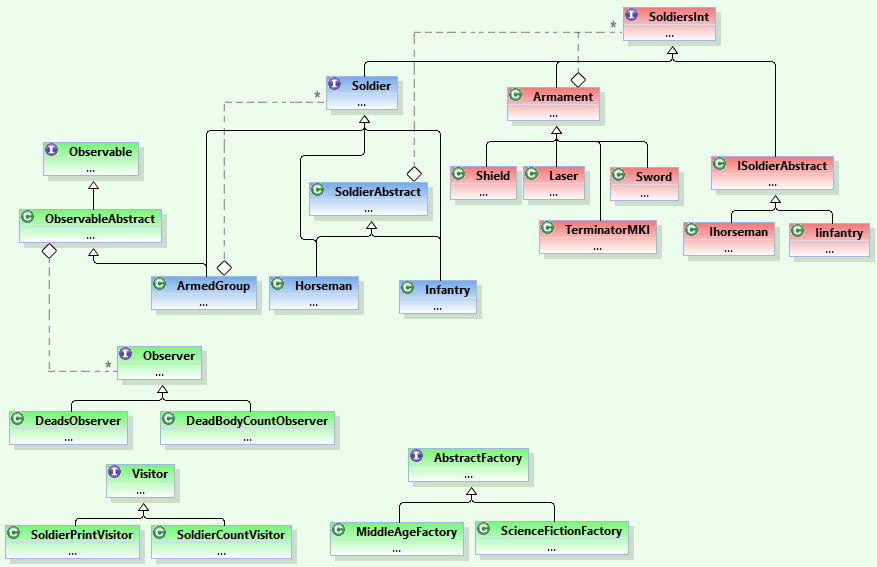
\includegraphics[width=11cm]{diagramme-classes-final}
\end{center}
    \caption{Diagramme de classes de l'application}
    \label{classes-final}
\end{figure}